\documentclass[11pt, oneside, titlepage]{article}
\usepackage[letterpaper, margin=2cm]{geometry}
\usepackage{MATH517}
\usepackage{Calculus}

\title{MATH 517 Finite Differences Homework 4}
\author{Caleb Logemann}

\begin{document}
\maketitle

%\lstinputlisting[language=Matlab]{H01_23.m}
\begin{enumerate}
    \item % #1 Done
        Which of the following Linear Multistep Methods are convergent?
        For the ones that are not, are they inconsistent, or not zero-stable,
        or both?
        \begin{enumerate}
            \item[(a)] % Done
                $U^{n+2} = \frac{1}{2} U^{n+1} + \frac{1}{2}U^n + 2k f(U^{n+1})$

                First from the book we see that the first two terms of the
                truncation error for any Linear Multistep method is
                \[
                    \tau = \frac{1}{k}\sum{j=0}{r}{\alpha_j} u(t_n) +
                    \sum{j=0}{r}{j\alpha_j - \beta_j} u'(t_n) + O(k)
                \]
                Therefore we see that for a method to be consistent, that is
                at least of order $k$, the following two equalities must be met.
                \begin{align*}
                    \sum{j=0}{r}{\alpha_j} &= 0 \\
                    \sum{j=0}{r}{j \alpha_j} = \sum{j=0}{r}{\beta_j}
                \end{align*}
                In these equtions $\alpha_j$ is the coefficient of $U^{n+j}$ and
                $\beta_j$ is the coefficient of $k f(U^{n+j})$ and $r$ is the
                number of steps.
                Also for a Linear Multistep method to be zero-stable, the root
                condition must be met, which states that the magnitude of the
                roots of the characteristic polynomial are less than or equal to
                one or strictly less than one if the root is repeated.
                These two conditions will be used to test all the following
                methods.

                The previous method can be rewritten as
                \[
                    U^{n+2} - \frac{1}{2}U^{n+1} - \frac{1}{2}U^n = 2k f(U^{n+1})
                \]
                For this method
                \begin{align*}
                    \sum{j=0}{r}{\alpha_j} &= 1 - \frac{1}{2} - \frac{1}{2} = 0 \\
                    \sum{j=0}{r}{j \alpha_j} &= 0 \times -\frac{1}{2} + 1 \times -\frac{1}{2} + 2 \times 1 = \frac{3}{2}
                    \sum{j=0}{r}{\beta_j} &= 2
                \end{align*}
                The second consistency condition is not satisfied, so this
                method is inconsistent.

                The characteristic polynomial for this method is
                \begin{align*}
                    \rho(\zeta) = \zeta^3 - \frac{1}{2}\zeta - \frac{1}{2} \\
                    \rho(\zeta) &= (\zeta - 1)\p{\zeta + \frac{1}{2}}
                \end{align*}
                The roots of this polynomial are $\zeta_1 = 1$ and
                $\zeta_2 = -\frac{1}{2}$.
                Neither of these roots are repeated and they both satisify
                $\abs{\zeta_j} \le 1$, therefore this method is zero-stable.

                Since this method is zero-stable but not consistent, this method
                is not convergent.

            \item[(b)] % Done
                $U^{n+1} = U^n$

                This method is equivalent to $U^{n+1} - U^n = 0$.
                \begin{align*}
                    \sum{j=0}{r}{\alpha_j} = 1 - 1 = 0 \\
                    \sum{j=0}{r}{j\alpha_j} &= 0(-1) + 1(1) = 1 \\
                    \sum{j=0}{r}{\beta_j} &= 0
                \end{align*}
                This method does not satisfy the consistency conditions.

                The characteristic polynomial for this method is
                \[
                    \rho(\zeta) = \zeta - 1.
                \]
                The root of this polynomial is $\zeta = 1$, this does satisfy
                the root condition, so the method is zero-stable.

                This method is zero-stable, but not consistent and therefore
                not convergent.

            \item[(c)] % Done
                $U^{n+4} = U^n + \frac{4}{3} k \p{f(U^{n+3}) + f(U^{n+2}) + f(U^{n+1})}$

                This method is equivalently
                $U^{n+4} - U^n = \frac{4}{3} k \p{f(U^{n+3}) + f(U^{n+2}) + f(U^{n+1})}$.
                \begin{align*}
                    \sum{j=0}{r}{\alpha_j} = 1 - 1 = 0 \\
                    \sum{j=0}{r}{j\alpha_j} &= 0(-1) + 4(1) = 4 \\
                    \sum{j=0}{r}{\beta_j} &= \frac{4}{3} + \frac{4}{3} + \frac{4}{3} = 4
                \end{align*}
                This method does satisfy both consistency conditions, and
                therefore is consistent.

                The characteristic polynomial for this method is
                \[
                    \rho(\zeta) = \zeta^4 - 1.
                \]
                The roots of this polynomial are $\zeta = 1, -1, i, -i$.
                None of these are repeated and all satisfy $\abs{\zeta} \le 1$,
                therefore the root condition is satisfied and this method is
                zero-stable.

                Since this method is both zero-stable and consistent, this
                method is convergent.

            \item[(d)] % Done
                $U^{n+3} + U^{n+2} - U^{n+1} - U^n = 2k\p{f(U^{n+2}) + f(U^{n+1})}$

                \begin{align*}
                    \sum{j=0}{r}{\alpha_j} = 1 + 1 - 1 - 1 = 0 \\
                    \sum{j=0}{r}{j\alpha_j} &= 0(-1) + 1(-1) + 2(1) + 3(1) = 4 \\
                    \sum{j=0}{r}{\beta_j} &= 2 + 2 = 4
                \end{align*}
                This method does satisfy both consistency conditions, and
                therefore is consistent.

                The characteristic polynomial for this method is
                \begin{align*}
                    \rho(\zeta) &= \zeta^3 + \zeta^2 - \zeta - 1 \\
                    \rho(\zeta) &= (\zeta - 1)(\zeta^2 + 2 \zeta + 1) \\
                    \rho(\zeta) &= (\zeta - 1)(\zeta + 1)^2
                \end{align*}
                The roots of this polynomial are $\zeta = 1, -1, -1$
                The root $\zeta = -1$ has multiplicity 2 and does not satisfy
                $\abs{\zeta} < 1$, therefore the root condition is not satisfied
                and the method is not zero-stable.
        \end{enumerate}

    \item % #2 Done
        \begin{enumerate}
            \item[(a)] % Done
                Determine the general solution to the linear difference equation
                $2U^{n+3} - 5U^{n+2} + 4U^{n+1} - U^n = 0$.
                % Hint one root of the characteristic polynomial is zeta = 1

                We know that the general solution to the linear difference
                equation is a linear combination of the roots of the
                characteristic polynomial.
                The characteristic polynomial for this linear difference
                equation is
                \begin{align*}
                    \rho(\zeta) &= 2\zeta^3 - 5\zeta^2 + 4\zeta - 1 \\
                    \rho(\zeta) &= (\zeta - 1)(2\zeta^2 - 3\zeta + 1) \\
                    \rho(\zeta) &= (\zeta - 1)^2(2\zeta - 1)
                \end{align*}
                The roots of this equation are $\zeta = 1, 1, \frac{1}{2}$.
                Since we have repeated roots the general solution to this
                difference equation is $U^n = c_1 + c_2 n + c_3 \frac{1}{2^n}$.

            \item[(b)] % Done
                Determine the solution to this difference equation with the
                starting values $U^0 = 11$, $U^1 = 5$, and $U^2 = 1$.
                What is the value of $U^{10}$?

                The 3 initial values create 3 equations in terms of
                $c_1, c_2, c_3$.
                \begin{align*}
                    11 &= c_1 + c_3 \\
                    5 &= c_1 + c_2 + \frac{1}{2}c_3 \\
                    1 &= c_1 + 2c_2 + \frac{1}{4}c_3
                \end{align*}
                These equations can be solved as follows.
                \begin{align*}
                    6 &= -c_2 + \frac{1}{2} c_3 \\
                    -4 &= c_2 - \frac{1}{4}c_3 \\
                    2 &= \frac{1}{4}c_3 \\
                    8 &= c_3 \\
                    c_1 &= 3 \\
                    c_2 &= 5 - 3 - 4 = -2 \\
                \end{align*}
                The solution is therefore
                \[
                    U^n = 3 - 2n + \frac{8}{2^n}
                \]
                The value of $U^{10}$ can then be found as follows
                \begin{align*}
                    U^{10} &= 3 - 2 \times 10 + \frac{8}{2^{10}} \\
                    &= -17 + \frac{8}{2^{10}} \\
                    &= -\frac{2175}{128}
                \end{align*}

            \item[(c)] % Done
                Consider the LMM
                \[
                    2U^{n+3} - 5U^{n+2} + 4U^{n+1} - U^n = k(\beta_0 f(U^n) + \beta_1 f(U^{n+1}))
                \]
                For what values of $\beta_0$ and $\beta_1$ is the local
                truncation error $O(k^2)$.

                In order for this method to be 2nd order the following two
                equations must be satistified.
                \begin{align*}
                    \sum{j = 0}{r}{j \alpha_j} &= \sum{j=0}{r}{\beta_j} \\
                    \sum{j=0}{r}{j^2 \alpha_j} &= \sum{j=0}{r}{j \beta_j} \\
                \end{align*}
                For this problem these two equations are equivalent to
                \begin{align*}
                    4 + 2(-5) + 3(2) &= 0 = \beta_0 + \beta_1 \\
                    4 + 4(-5) + 9(2) &= 2 = \beta_1 \\
                    \beta_0 &= -2
                \end{align*}
                Thus for this method to be second order $\beta_0 = -2$ and
                $\beta_1 = 2$.

            \item[(d)] % Done
                Suppose you use the values of $\beta_0$ and $\beta_1$ just
                determined in this LMM. Is this a convergent method?

                No this method is not convergent, because the roots of the
                characteristic polynomial as shown in part (a) are
                $\zeta = 1, 1, \frac{1}{2}$.
                The root $\zeta = 1$ has multiplicity 2 and does not satisfy
                $\abs{\zeta} < 1$.
                Therefore the root condition is not satisfied and the method is
                not zero-stable.
                This implies that the method is not convergent.
        \end{enumerate}

    \item % #3
        Consider the so-called $\theta$-method for $u'(t) = f(u(t))$,
        \[
            U^{n+1} = U^n + k\br{(1 - \theta)f(U^n) + \theta f(U^{n+1})},
        \]
        where $\theta$ is a fixed parameter.
        \begin{enumerate}
            \item[(a)]
                Show that the method is A-stable for $\theta \ge \frac{1}{2}$.

                A method is A-stable if the region of absolute stability
                contains the entire left-half complex plane.
                The stability region for this method can be found as follows.
                The stability polynomial for this method is
                \begin{align*}
                    \pi(\zeta; z) &= (-1 - z(1 - \theta)) + (1 - z\theta)\zeta
                    \intertext{The root of this polynomial is}
                    \zeta &= \frac{-1 - z + z\theta}{1 - z\theta} \\
                    \zeta &= -1 + \frac{z}{z \theta - 1}
                    \intertext{In order for the root condition to be met}
                    \abs{-1 + \frac{z}{z \theta - 1}} \le 1 \\
                    \p{-1 + \frac{z}{z \theta - 1}}\p{-1 + \frac{z^*}{z^* \theta - 1}} \le 1 \\
                    1 - \frac{z}{z \theta - 1} - \frac{z^*}{z^* \theta - 1} + \frac{zz^*}{(z\theta - 1)(z^*\theta - 1)} \le 1 \\
                    \frac{-z(z^*\theta - 1) - z^*(z\theta - 1) + zz^*}{(z \theta - 1)(z^* \theta - 1)} \le 0 \\
                    \frac{(1 - 2\theta)zz^* + z^* + z}{zz^* \theta^2 -\theta (z^* + z) + 1} \le 0 \\
                    \frac{(1 - 2\theta)zz^* + 2\operatorname{Re}(z)}{zz^* \theta^2 - 2\theta\operatorname{Re}(z) + 1} \le 0 \\
                    \intertext{If $\operatorname{Re}(z) \le 0$, then $zz^* \theta^2 - 2\theta\operatorname{Re}(z) + 1 > 0$ so}
                    (1 - 2\theta)zz^* + 2\operatorname{Re}(z)\le 0 \\
                \end{align*}
                This equality is met if $\theta \ge \frac{1}{2}$, since $zz^* > 0$
                and $\operatorname{Re}(z) < 0$.
                Therefore for $\theta \ge \frac{1}{2}$ the root condition is
                met for all $z$ such that $\operatorname{Re}(z) \le 0$.
                This means that the region of stability includes the left-half
                plane for $\theta \ge \frac{1}{2}$.
                Thus this method is A-stable for $\theta \ge \frac{1}{2}$.

            \item[(b)]
                Plot the stability region, S, for
                $\theta = 0, \frac{1}{4}, \frac{1}{2}, \frac{3}{4}, 1$ and
                comment how the stability region will look for other values of
                $\theta$.

                Plots of the stability regions are shown below.
                For values of $\theta < .5$, the region of stability is a circle
                in the left half plane whose radius is increasing as $\theta$ approaches
                $.5$.
                At $\theta = .5$ the region of stability is the left-half plane.
                For $\theta > .5$ the region of stability is everything
                except a circle in the right-half plane.
                This circle's radius is decreasing as $\theta$ approaches 1.
                \begin{center}
                   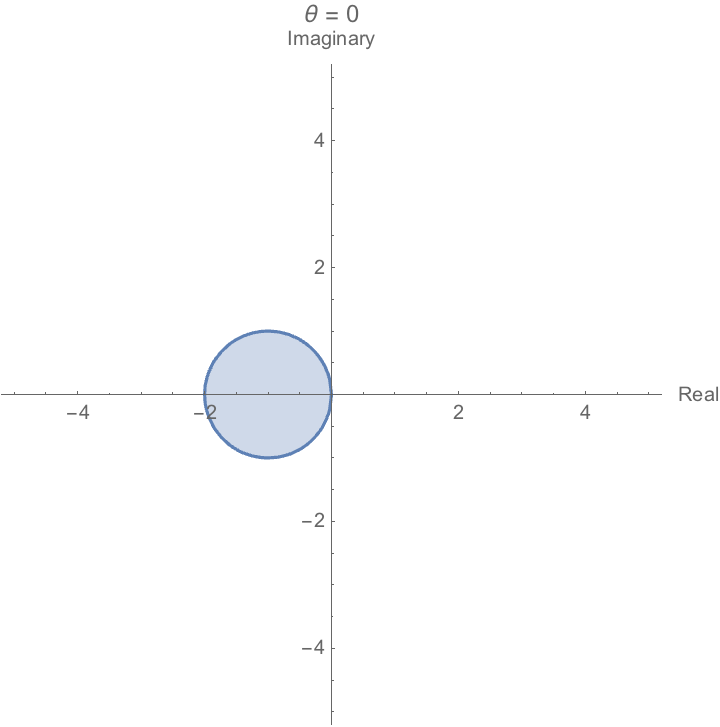
\includegraphics[scale=.3]{Figures/04_3_1.png}
                   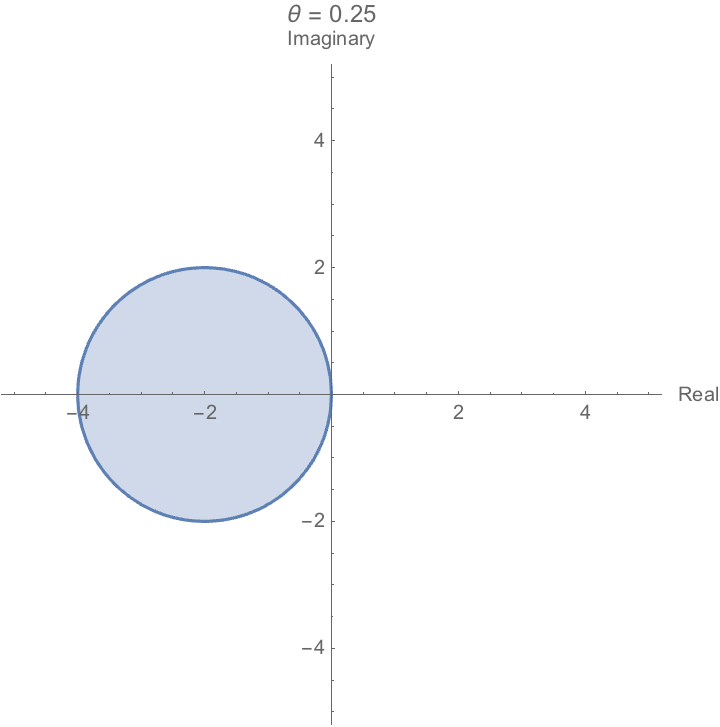
\includegraphics[scale=.3]{Figures/04_3_2.png}
                   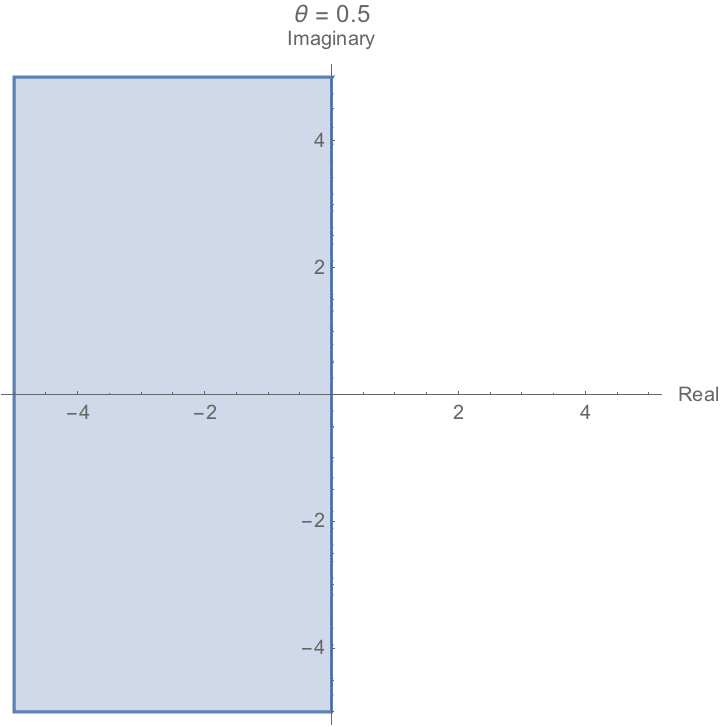
\includegraphics[scale=.3]{Figures/04_3_3.png}
                   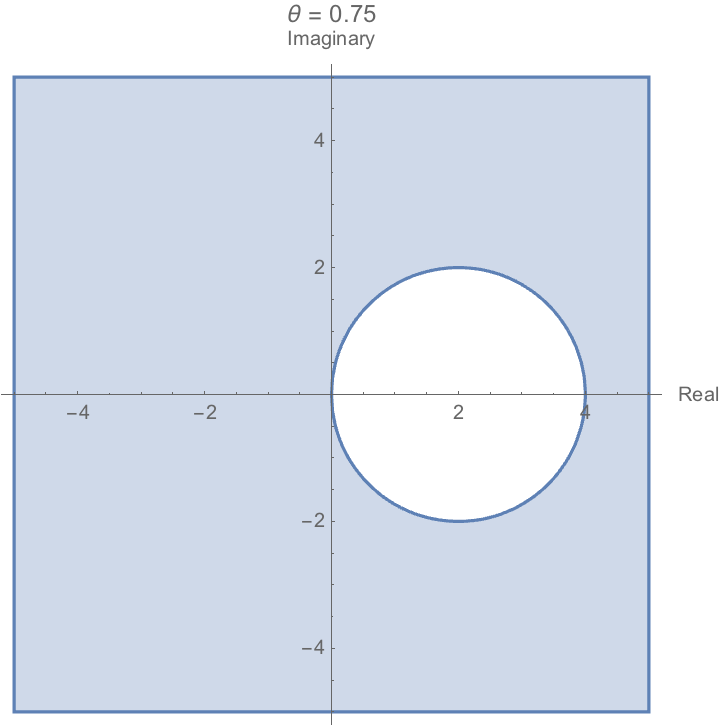
\includegraphics[scale=.3]{Figures/04_3_4.png}
                   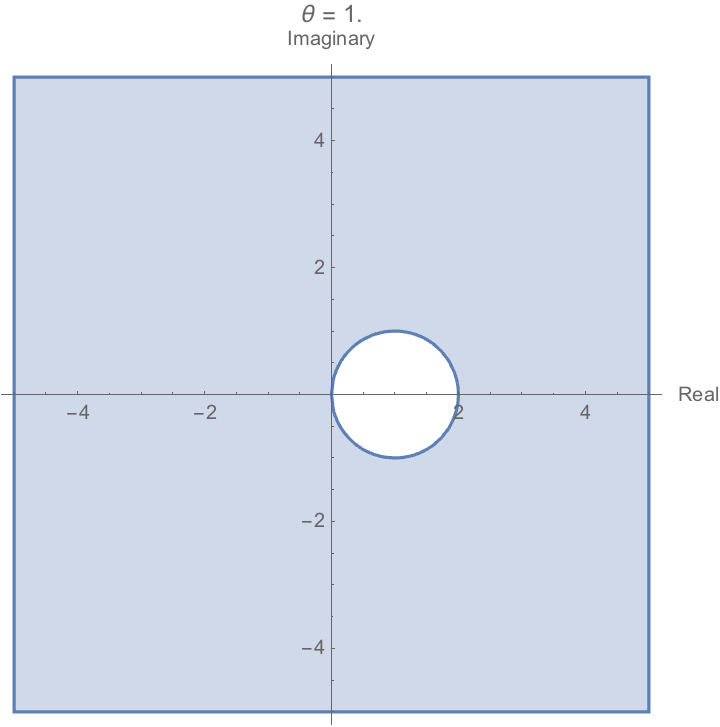
\includegraphics[scale=.29]{Figures/04_3_5.png}
                \end{center}

        \end{enumerate}

    \item % #4
        \begin{enumerate}
            \item[(a)]
                On the attached mathematica printout it is shown that this
                method for $f(u) = \lambda u$, that this method is equivalent
                to
                \[
                    U^{n+1} = \p{\frac{12 + 6 k\lambda + (k\lambda)^2}{12 - 6k\lambda + (k\lambda)^2}}U^n.
                \]
                This is equivalent to
                \[
                    U^{n+1} = e^{k \lambda} U^n - \frac{(k \lambda)^5}{720} + O(k^6).
                \]
                Thus the one-step error is order $k^5$, and the local
                truncation error is order $k^4$.


            \item[(b)]
                We showed in part (a) that the stability function was
                $R(z) = \frac{12 + 6z + z^2}{12 - 6z + z^2}$.
                In order for this method to be A-stable $\abs{R(z)} \le 1$
                for all $z$ such that $\operatorname{Re}(z) \le 1$.

                From the picture on the mathematica printout we can see that this
                condition is satisfied, so this method is A-stable.

            \item[(c)]
                This method is not L-stable because the limit of $R(z)$ as
                $z \to \infty$ along the real axis is 1.
                In other words
                \[
                    \lim{z \to \infty}{R(z)} = 1.
                \]
                Thus this method is not L-stable.
        \end{enumerate}
\end{enumerate}
\end{document}
